\documentclass[slidetop,11pt]{beamer}
%
% Ces deux lignes {\`a} d{\'e}commenter pour sortir 
% le texte en classe article
% \documentclass[class=article,11pt,a4paper]{beamer}
% \usepackage{beamerbasearticle}

% Packages pour les fran\c{c}ais
%
\usepackage[T1]{fontenc} 
\usepackage[latin1]{inputenc}
\usepackage[frenchb]{babel}
% pour un pdf lisible {\`a} l'{\'e}cran si on ne dispose pas 
% des fontes cmsuper ou lmodern
%\usepackage{lmodern}
\usepackage{aeguill}

% Pour afficher le pdf en plein ecran
% (comment{\'e} pour imprimer les transparents et pour les tests)
%\hypersetup{pdfpagemode=FullScreen}

% Red{\'e}finit la couleur de fond pour imprimer sur transparents
%\xdefinecolor{fondtexte}{rgb}{1,1,1}     % blanc

% commande differente pour les couleurs nomm{\'e}es - de base
%\colorlet{coultexte}{black} 

% -------------- Fioritures de style -------------
% Fait afficher l'ensemble du frame 
% en peu lisible (gris clair) d{\`e}s l'ouverture
\beamertemplatetransparentcovered

% Supprimer les icones de navigation (pour les transparents)
\setbeamertemplate{navigation symbols}{}

% Mettre les icones de navigation en mode vertical (pour projection)
% \setbeamertemplate{navigation symbols}[vertical]

\usetheme{Warsaw}

%------------ fin style beamer -------------------

% Faire appara{\^i}tre un sommaire avant chaque section
% \AtBeginSection[]{
%   \begin{frame}
%   \frametitle{Plan}
%   \medskip
%   %%% affiche en d{\'e}but de chaque section, les noms de sections et
%   %%% noms de sous-sections de la section en cours.
%   \small \tableofcontents[currentsection, hideothersubsections]
%   \end{frame} 
% }

% ----------- Contenu de la page de titre --------
\title{Recruter en informatique}
\subtitle{Les mauvaises id{\'e}es... et les bonnes !} 
\author{Gabriel Chandesris}
\institute{\emph{Data Engineer / Dev Senior / ...}}
%% \date{\today} \date{19 mai 2020} %% \date{\today} %% \date{03 Janvier 2018}
\logo{
\includegraphics[height=0.5cm]{img/logo_glider.png}}

% ----------- Nom des diff{\'e}rentes parties --------

%% Mis au fur et {\`a} mesure...

% ----------- Autres Packages --------

\usepackage{tikzpeople}

\usepackage{JeuxCartes}

% ------------------------------------------------
% -------------   D{\'e}but document   ---------------
% ------------------------------------------------
\begin{document}
%--------- {\'e}criture de la page de titre ----------
% avec la commande frame simplifi{\'e}e
%% \frame[plain]{ \titlepage }
\frame[plain]{ \titlepage %
		\MainCartesJeuAleatoire[TypeJeu=Uno,Eventail,Hauteur=2.5,EspH=0,EspV=0.1]{5}
		\MainCartesJeuAleatoire[TypeJeu=Poker,Eventail,Hauteur=2.5,EspH=0,EspV=0.1]{5}
		\MainCartesJeu[TypeJeu=Tarot,Inverse,Eventail,Hauteur=3.0,EspH=0,EspV=0.1]%
			{Exc § 1AT § 3AT § 7AT § 21AT}
} 
%

%------------------ Sommaire ---------------

\begin{frame}
	\frametitle{Sommaire}
	\small \tableofcontents[hideallsubsections]
\end{frame} 

\section{Recrutement en informatique, une introduction}
\begin{frame}
	\frametitle{Recrutement en informatique, une introduction}
	\tableofcontents[sections=1,currentsection,subsectionstyle=show/shaded/hide] %% sectionstyle=hide/hide,
\end{frame}

\subsection{Introduction}
\begin{frame}
	\frametitle{Introduction}
	\begin{itemize}
		\item L'objectif ici est seulement de recenser une liste de pratiques ; 
		\item Enlever les clich{\'e}s RH sur les informaticiens, d{\'e}veloppeurs, ing{\'e}nieurs en informatique... ; 
		\item Faire sauter les soucis principaux du recrutement (nombre de candidats, turn-over, refus de contact...) ;
		\item Faire {\'e}voluer les mentalit{\'e}s (divas des deux bords, sexisme, racisme, LGBTphobies...) ; 
		\item ...  
	\end{itemize}
\end{frame}

\begin{frame}
	\frametitle{Introduction (visuelle)}

	\begin{tikzpicture}
		% \draw [very thin, gray] (0,0) grid (11,7);
		% \node[person,minimum size=1.5cm] (B) at (0,4) {A Person};
		
		\node[name=alice,alice,minimum size=1.5cm] (A) at (1,6) {Alice};
		\node[name=bob,bob,mirrored,minimum size=1.5cm] (B) at (10,5) {Bob};
		
		\node[draw,text width=5cm,text justified,minimum width=5.5cm,minimum height=1cm,font=\tiny,fill=yellow!35]
			at (5,6) {Salut ! Tu me files ton '06', qu'on fasse un call ?};
		\node[draw,text width=3cm,text justified,minimum width=3.5cm,minimum height=1cm,font=\tiny,fill=green!35]
			at (7,5) {D'abord que proposez-vous, par {\'e}crit ? (pas assez intimes)};
		\node[draw,text width=5cm,text justified,minimum width=5.5cm,minimum height=1cm,font=\tiny,fill=yellow!35]
			at (5,4) {C'est super urgent pour un "grand compte", avec une super ambiance  et super avantages !};
		\node[draw,text width=3cm,text justified,minimum width=3.5cm,minimum height=1cm,font=\tiny,fill=green!35]
			at (7,3) {Et sinon, pour le reste ? ( secteur d'activit{\'e}, localisation, r{\'e}mun{\'e}rations...) ?};
		\node[draw,text width=5cm,text justified,minimum width=5.5cm,minimum height=1cm,font=\tiny,fill=yellow!35]
			at (5,2) {Comment \c{c}a, ma description g{\'e}n{\'e}rique ne suffit pas ? C'est pour du bancaire {\`a} Champignac-En-Cambrousse, selon pofil !};
		\node[draw,text width=3cm,text justified,minimum width=3.5cm,minimum height=1cm,font=\tiny,fill=green!35]
			at (7,1) {Non ! (pas de descriptif, loin, pas assez bien pay{\'e}...) };
	\end{tikzpicture}

\end{frame}

\subsection{Mauvaises id{\'e}es, pr{\'e}jug{\'e}s...}
\begin{frame}
	\frametitle{Mauvaises id{\'e}es, pr{\'e}jug{\'e}s...}
	\begin{itemize}
		\item Recrutement uniquement sur mots-clefs et ignorer le contenu ; 
		\item Que des femmes pour recruter des hommes~\newline
			("LinkedIn est un Tinder invers{\'e}. ") ; 
		\item Recrutement sur "gadget" : comp{\'e}tences, ann{\'e}es d'exp{\'e}riences... et le sens ?
		\item Recherche de "M{\^a}les Alphas C{\'e}libataires Sans Enfants" ; 
		\item R{\'e}f{\'e}rences ? Quelles r{\'e}f{\'e}rences ? Pourquoi ?
		\item Pr{\'e}sentation g{\'e}n{\'e}rique, "recrutement sur profil", "grille de salaire"... ; et au-del{\`a} ? 
		\item "Le digital : {\`a} manipuler avec doigt{\'e} !" : num{\'e}rique !
		\item Et la culture associ{\'e}e... 
	\end{itemize}
\end{frame}

\begin{frame}
	\frametitle{Mauvaises id{\'e}es, pr{\'e}jug{\'e}s... : non-recrutement !}

	\begin{tikzpicture}
		% \draw [very thin, gray] (0,0) grid (11,7);
		% \node[person,minimum size=1.5cm] (B) at (0,4) {A Person};
		
		\node[name=businessman,businessman,minimum size=1.5cm] (A) at (1,6) {Commercial};
		\node[name=charlie,charlie,mirrored,minimum size=1.5cm] (B) at (10,5) {Charlie};
		
		\node[draw,text width=5cm,text justified,minimum width=5.5cm,minimum height=1cm,font=\tiny,fill=yellow!35]
			at (5,6) {Salut ! Tu as 5 {\`a} 10 ans d'exp{\'e}riences sur SuperTechnoXYZ ? et sur SuperTechnoXYZ-script ?};
		\node[draw,text width=3cm,text justified,minimum width=3.5cm,minimum height=1cm,font=\tiny,fill=green!35]
			at (7,5) {Je connais bien "SuperTechnoXYZ", \c{c}a existe depuis 18 mois ! "SuperTechnoXYZ"-script n'a rien {\`a} voir !};
		\node[draw,text width=5cm,text justified,minimum width=5.5cm,minimum height=1cm,font=\tiny,fill=yellow!35]
			at (5,4) {Le client veut absolument minimum 5 ans d'exp{\'e}rience sur SuperTechnoXYZ !};
		\node[draw,text width=3cm,text justified,minimum width=3.5cm,minimum height=1cm,font=\tiny,fill=green!35]
			at (7,3) {C'est moi qui ai cr{\'e}{\'e} "SuperTechnoXYZ" (sur mon temps libre, pour faciliter le travail).};
		\node[draw,text width=5cm,text justified,minimum width=5.5cm,minimum height=1cm,font=\tiny,fill=yellow!35]
			at (5,2) {Votre profil ne convient pas du tout aux besoins ! Et il faut aussi {\^e}tre d'un signe astrologique pr{\'e}cis, et sans famille !};
		\node[draw,text width=3cm,text justified,minimum width=3.5cm,minimum height=1cm,font=\tiny,fill=green!35]
			at (7,1) {Est-ce que vous comprenez r{\'e}ellement ces besoins ?};
	\end{tikzpicture}

\end{frame}

\subsection{Bonnes id{\'e}es (?)}
\begin{frame}
	\frametitle{Bonnes id{\'e}es (?)}
	\begin{itemize}
		\item Instruisez-vous, renseignez-vous, oubliez vos clich{\'e}s...
		\item Communiquer directement les enjeux (missions, r{\'e}mun{\'e}ration, conditions de travail...) ;
		\item Environnement bienveillant, tol{\'e}rant, ouvert, inclusif, divers...
		\item Distinction Vie Pro et Vie Perso...
		\item Reconnaissance et assurer l'avenir : {\^e}tre correct avec tout le monde, y compris les contractuels / prestataires / stagiaires...
		\item Une {\'e}quipe, cela se construit, et il n'y a pas d'argent magique, ni de management magique...
		%% \item ...
	\end{itemize}
	
	\emph{Note : une obligation l{\'e}gale sociale n'est pas un avantage de l'entreprise (mutuelle, transports, cong{\'e}s et RTT...). } 
\end{frame}

%%%%% %%%%% %%%%% %%%%% %%%%% 

\section{Interm{\`e}de (Pop-)Culture}
\begin{frame}
	\frametitle{Interm{\`e}de (Pop-)Culture}
	\tableofcontents[sections=2,currentsection,subsectionstyle=show/shaded/hide] %% sectionstyle=hide/hide,
\end{frame}

\def\titleSubSectionEntreprisesFictives{Quelques entreprises fictives}
\subsection{\titleSubSectionEntreprisesFictives }
\begin{frame}
	\frametitle{\titleSubSectionEntreprisesFictives  (1)}
	
	\begin{center}
		
\includegraphics[width=0.65\textwidth]{img/191816865_144589207657338_3945577351766051195_n.png}~\\
		\emph{Quelques entreprises de fiction / fictives~\newline certaines pr{\'e}sentes sur LinkedIn !}
	\end{center}
	
\end{frame}

\begin{frame}
	\frametitle{\titleSubSectionEntreprisesFictives  (2)}
	
	\begin{minipage}{0.45\textwidth}
		
\includegraphics[width=0.95\textwidth]{img/191743009_5940031996070069_3438760338176067873_n.jpg}~\\
		\emph{Wallace Corporation~\newline (Film "BladeRunner 2049")}~\\
	\end{minipage} \hfill \begin{minipage}{0.45\textwidth}
		
\includegraphics[width=0.95\textwidth]{img/191939426_5940071632732772_6985810412209495092_n.jpg}~\\
		\emph{InGen~\newline (Franchise "Jurassic Park")}~\\
	\end{minipage}
	
\end{frame}

\begin{frame}
	\frametitle{\titleSubSectionEntreprisesFictives  (3)}
	
	\begin{minipage}{0.45\textwidth}
		
\includegraphics[width=0.95\textwidth]{img/192261268_4163395560408024_2949464129711293154_n.jpg}~\\
		\emph{Skynet~\newline (Film "Terminator")}~\\
	\end{minipage} \hfill \begin{minipage}{0.45\textwidth}
		
\includegraphics[width=0.95\textwidth]{img/zOrg_cropped-part1.jpg}~\\
		\emph{zOrg Industries$^{TM}$~\newline ("Le Cinqui{\`e}me {\'E}l{\'e}ment")}~\\
	\end{minipage}
	
\end{frame}

\begin{frame}
	\frametitle{\titleSubSectionEntreprisesFictives  (4)}
	
	\begin{minipage}{0.45\textwidth}
		
\includegraphics[width=0.95\textwidth]{img/Corpo_segatari.png}~\\~\\
		\emph{SEGATARI~\newline (JdR "CyberPunk 2020"~\newline JV "CyberPunk 2077")}~\\
	\end{minipage} \hfill \begin{minipage}{0.45\textwidth}
		
\includegraphics[width=0.95\textwidth]{img/Logo_Arasaka_(rouge)_cropped-part1.png}~\\
		\emph{Arasaka Corporation~\newline (JdR "CyberPunk 2020"~\newline JV "CyberPunk 2077")}~\\
		%% 
\includegraphics[width=0.95\textwidth]{img/Logo_Raven_Microcybernetics.png}~\\
		%% \emph{Raven Microcybernetics~\newline (JdR "CyberPunk 2020", JV "CyberPunk 2077")}~\\
	\end{minipage}
	
\end{frame}

\begin{frame}
	\frametitle{\titleSubSectionEntreprisesFictives  (5)}
	
	\begin{minipage}{0.45\textwidth}
		
\includegraphics[width=0.95\textwidth]{img/tessier_ashpool_sa_cover_cropped-part1.jpeg}~\\
		\emph{Tessier-Ashpool SA~\newline (Roman "Neuromancien")}~\\
	\end{minipage} \hfill \begin{minipage}{0.45\textwidth}
		
\includegraphics[width=0.95\textwidth]{img/ApertureLaboratories.jpeg}~\\
		\emph{Aperture Laboratories~\newline (JV "Portal" \& "Portal 2")}~\\
	\end{minipage}
	
\end{frame}

\begin{frame}
	\frametitle{Quelques entreprises (5)}
	
	\begin{minipage}{0.45\textwidth}
		
\includegraphics[width=0.95\textwidth]{img/StarkIndustries_cropped-part1.jpeg}~\\
		\emph{Stark Industries~\newline (Franchise "Marvel")}~\\
	\end{minipage} \hfill \begin{minipage}{0.45\textwidth}
		
\includegraphics[width=0.95\textwidth]{img/WaynesEnterprises.png}~\\
		\emph{Wayne Enterprises~\newline (Franchise "DC")}~\\
	\end{minipage}
	
\end{frame}

\def\titleSubSectionDefinitionPopCulture{D{\'e}finition (?) de la "Pop-Culture"}
\subsection{\titleSubSectionDefinitionPopCulture }
\begin{frame}
	\frametitle{\titleSubSectionDefinitionPopCulture }
	\footnotesize 
	Ce qui sort de la culture classique apprise {\`a} l'{\'e}cole (auteurs reconnus...) et d'un r{\'e}f{\'e}rentiel "norm{\'e}" / normatif. 
	\begin{columns}[T]
	\begin{column}[T]{5.0cm}
		\begin{block}{Supports {\'e}crits et assimil{\'e}s}
			\begin{itemize}
				\item Livres, films, jeux vid{\'e}os (et autres supports) ; 
				\item Curiosit{\'e} : Fantasy, Science-Fiction et (sous-)divisions (CyberPunk...)
				\item Anim{\'e}, Manga...
				\item Tolkien (Hobbit, Anneaux), Asimov (Robots, Fondation), Herbert (Dune)... 
				\item JdR (non limitatif {\`a} DnD !) : Vampire, Cthulhu, ... 
				%% \item Jeux vid{\'e}os ("The cake is a lie !", "Too Many Secrets"...)
			\end{itemize}
		\end{block}
	\end{column}
	\begin{column}[T]{5.0cm}
		\begin{block}{Memes culturels}
			\begin{itemize}
				\item Besoin de cr{\'e}ativit{\'e} ! Et d'abstraction ! Moyens d'existence et d'expression ! ; 
				\item L{\'e}gendes Urbaines (CreepyPasta, et classiques) ; 
				\item Culture du 'meme' (message visuel et {\'e}crit) ; 
				\item R{\'e}f{\'e}rences {\`a} des {\'e}l{\'e}ments culturels partag{\'e}s ; 
				\item Cultures 'alternatives' (M{\'e}tal, Gamer, LGBTQI+, Goth...) ; 
			\end{itemize}
		\end{block}
	\end{column}
	\end{columns}~\\
\end{frame}

%%%%% %%%%% %%%%% %%%%% %%%%% 

\section{Recrutement en informatique : les mauvaises pratiques}
\begin{frame}
	\frametitle{Recrutement en informatique : les mauvaises pratiques}
	\tableofcontents[sections=3,currentsection,subsectionstyle=show/shaded/hide] %% sectionstyle=hide/hide,
\end{frame}

\subsection{Pr{\'e}jug{\'e}s "techniques"}
\begin{frame}
	\frametitle{Pr{\'e}jug{\'e}s "techniques"}
	\begin{minipage}{0.82\textwidth}
		\begin{itemize}
			\item Aspects techniques peu attirants... \c{C}a d{\'e}pend pour qui ! ; 
			\item Milieu Geek / Nerd / "Alternatif" / LGBTQIA+ / (?)... ; %% Mascu ?
			\item Terminologie magique ("digital / num{\'e}rique", acronymes, "Java / JavaScript", "Shell / PowerShell", le terminal "Matrix"...) ; 
			\item Informatique magique ("c'est simple", parfois non, apprentissage et dipl{\^o}mes ! ) ; 
			\item[] 
			\item Comme tout, \c{c}a s'apprend ! Au moins une culture minimale sur les acronymes, des {\'e}l{\'e}ments de (pop-)culture... 
		\end{itemize}
	\end{minipage} \hfill \begin{minipage}{0.14\textwidth}
		\begin{tikzpicture}
			\node[name=alice,alice,mirrored,monitor,minimum size=0.75cm] at (0,7) {};
			\node[name=nun,nun,mirrored,monitor,minimum size=0.75cm] at (0,6) {};
			\node[name=nurse,nurse,mirrored,monitor,minimum size=0.75cm] at (0,5) {};
			\node[name=groom,groom,mirrored,monitor,minimum size=0.75cm] at (0,4) {};
			\node[name=sailor,sailor,mirrored,monitor,minimum size=0.75cm] at (0,3) {};
			\node[name=graduate,graduate,mirrored,monitor,minimum size=0.75cm] at (0,2) {}; 
		\end{tikzpicture}
	\end{minipage} 
\end{frame}

\subsection{Soucis de recrutement}
\begin{frame}
	\frametitle{Soucis de recrutement}
	\begin{itemize}
		\item Turn-Over, concurrence des recruteurs (ESN / SS2I), harc{\`e}lement de contact... 
		\item Que des femmes pour recruter des hommes, ou presque !~\newline
		("LinkedIn est un Tinder invers{\'e}. ") ; 
		\item Recherche de "M{\^a}les Alphas C{\'e}libataires Sans Enfants" ; ...
		\item Recrutement uniquement sur mots-clefs et ignorer le contenu ("c'est quoi XYZ ?") ; 
		\item Recrutement sur "gadget" : comp{\'e}tences, ann{\'e}es d'exp{\'e}riences... et le sens ?
		\item Recrutement sur "exp{\'e}rience biais{\'e}e" : Cinq ans d'exp{\'e}riences pour une technologie / technique existant de puis deux ans ?!
	\end{itemize}
\end{frame}

\subsection{Lev{\'e}es de drapeaux rouges !}
\begin{frame}
	\frametitle{Lev{\'e}es de drapeaux rouges !}
	\begin{itemize}
		\item Soci{\'e}t{\'e} de Service en Informatique ("A*" / externalisations) ; 
		\item Pr{\'e}sentation comme avantages ce qui rel{\`e}ve du l{\'e}gal (cong{\'e}s pay{\'e}s, tickets restaurants, remboursement des transports...) ; 
		\item Ambiance(s) toxique(s) : management inadapt{\'e}, "mascus et alphas", prestataires / consultants...
		\item Recrutement sur profil (bloquer la concurrence ?) ; 
		\item Recrutement en comp{\'e}tition (fa\c{c}on consultant commercial) ; 
		\item Conditions : OpenSpace avec plus de 10 personnes, T{\'e}l{\'e}Travail limit{\'e}, "argent magique"...
		\item ... 
	\end{itemize}
\end{frame}

\subsection{Prise de contact avec un(e) candidat(e) ?}
\begin{frame}
	\frametitle{Prise de contact avec un(e) candidat(e) ?}
	\begin{itemize}
		\item {\'E}viter de lire son profil LinkedIn / son CV (au-del{\`a} s{\'e}lection) ; 
		\item \emph{Mettez votre mauvaise pratique ici !} ; 
		\item Contacter fortement et rapidement par t{\'e}l{\'e}phone en ignorant le r{\'e}pondeur (ou autre outil, par exemple email...) ;  
		\item MESSAGE G{\'E}N{\'E}RIQUE OU AUTOMATIQUE :~\newline pour avoir des candidats fant{\^o}mes ("ghosting") ; 
		\item MESSAGE G{\'E}N{\'E}RIQUE OU AUTOMATIQUE :~\newline si vous {\^e}tes disponible soirs et WeekEnd !
		\item ... 
	\end{itemize}
\end{frame}

\subsection{Mauvais Cas Pratique 1}
\begin{frame}
	\frametitle{Mauvais Cas Pratique 1 : la chaine des commerciaux}
	\begin{itemize}
		%% https://www.linkedin.com/posts/rudy-onfroy_message-re%C3%A7u-sur-linkedin-votre-profil-activity-7200746078479024128-e8Vn
		\item \textbf{\emph{Exp{\'e}rience v{\'e}cue, ne reproduisez pas chez vous !}}
		\item "Votre profil correspond parfaitement {\`a} un poste que nous avons {\`a} pourvoir. J'aimerais beaucoup discuter avec vous de cette superbe opportunit{\'e}."
		\item Oui, pourquoi pas, on peut prendre RDV pour que j'en apprenne plus sur votre entreprise et sur la mission.
		\item \underline{Pendant l'entretien :} "Pourquoi avez-vous d{\'e}cid{\'e} de postuler chez nous ? Qu'est-ce qui vous int{\'e}resse dans notre entreprise ? Pourquoi pensez-vous {\^e}tes la meilleure personne pour ce poste ?"
		\item \underline{R{\'e}ponse du candidat :} "C'est vous qui m'avez contact{\'e}, je ne connaissais m{\^e}me pas votre existence hier !"
	\end{itemize}
\end{frame}

\subsection{Mauvais Cas Pratique 2}
\begin{frame}
	\frametitle{Mauvais Cas Pratique 2 : Tout dans la m{\^e}me soci{\'e}t{\'e} !}
	\begin{itemize}
		%% https://www.linkedin.com/posts/pb42_on-a-quune-chance-de-faire-bonne-impression-activity-7199329366139424768-fXHX
		\item \textbf{\emph{Exp{\'e}rience v{\'e}cue, ne reproduisez pas chez vous !}}
		\item[] 
		\item "On n'a qu'une chance de faire bonne impression,~\newline c{\^o}t{\'e} recruteur !"~\newline
		\begin{tikzpicture}
			\node[name=jester,jester,mirrored,evil,minimum size=0.75cm] at (0,0) {};
			\node[name=criminal,criminal,good,female,minimum size=0.75cm] at (2.5,0) {};
			\node[name=santa,santa,good,evil,minimum size=0.75cm] at (5,0) {};
			\node[name=nun,nun,female,good,evil,minimum size=0.75cm] at (7,0) {};
			\node[name=maninblack,maninblack,mirrored,good,evil,minimum size=0.75cm] at (9,0) {};
		\end{tikzpicture}
		\item Entretiens {\`a} r{\'e}p{\'e}tition (occuper le terrain ?) aux "candidats" ; 
		\item Tests d{\'e}pass{\'e}s : technique d{\'e}su{\`e}te ; 
		\item Tests sans rapport avec le poste propos{\'e} ;  
		\item D{\'e}marche "{\`a} l'instinct" plut{\^o}t que de documentation ; 
		%% \item ... 
	\end{itemize}
\end{frame}

%%%%% %%%%% %%%%% %%%%% %%%%% 

\section{Recrutement en informatique : pour faire mieux}
\begin{frame}
	\frametitle{Recrutement en informatique : pour faire mieux}
	\tableofcontents[sections=4,currentsection,subsectionstyle=show/shaded/hide] %% sectionstyle=hide/hide,
\end{frame}

\subsection{Bonnes id{\'e}es (1)}
\begin{frame}
	\frametitle{Bonnes id{\'e}es (1)}
	\begin{itemize}
		\item Instruisez-vous, renseignez-vous : culture ? technicit{\'e} ? industrie ? ambiance ?...
		\item Communiquer directement les enjeux (missions, conditions de travail, r{\'e}mun{\'e}ration...) ;
		\item Environnement bienveillant, tol{\'e}rant, ouvert, inclusif, diversit{\'e}. % , t{\'e}l{\'e}travail...
		\item Distinction Vie Pro et Vie Perso...
		\item Reconnaissance et assurer l'avenir : {\^e}tre correct avec tout le monde, y compris les contractuels / prestataires / stagiaires...
		\item Une {\'e}quipe, cela se construit, et il n'y a pas d'argent magique, ni de management magique...
		\item Aller chercher les candidats (et s'int{\'e}resser {\`a} leur CV, leur parcours pro, contraintes {\'e}ventuelles)...
	\end{itemize} 
\end{frame}

\subsection{Bonnes id{\'e}es (2)}
\begin{frame}
	\frametitle{Bonnes id{\'e}es (2)}
	\begin{itemize}
		\item Poste sur lequel il y a recrutement : les enjeux doivent {\^e}tre donn{\'e}s (premier contact ou entretien qui suit) ;~\newline
		$\Rightarrow$ Pr{\'e}parez ces donn{\'e}es en amont : sinon, c'est du temps perdu pour tout le monde !
		
		\item Environnement de travail inclusif, et diversit{\'e}... ~\newline
		Pas de concessions ici : mal {\`a} l'aise en entretien ou apr{\`e}s, le ressenti a des cons{\'e}quences pas forc{\'e}ments visibles imm{\'e}diatement.
		
		\item Au-del{\`a} de la passion : des individus !~\newline
		{\'E}vitez quand m{\^e}me les divas et / ou les personnes qui se n{\'e}gligent (franchise et direct l{\`a}-dessus si le cas se pr{\'e}sente). 
	\end{itemize} 
\end{frame}

\subsection{Bonnes id{\'e}es (3)}
\begin{frame}
	\frametitle{Bonnes id{\'e}es (3)}
	\begin{itemize}
		\item Faites propositions concr{\`e}tes sur profils susceptibles de r{\'e}pondre avec les crit{\`e}res suivants de proposition :
		\begin{itemize}
			\item Mission int{\'e}ressante (pr{\'e}ciser le contexte autant que possible, t{\^a}ches {\`a} accomplir...) ; 
			\item Adaptation au profil (exemple : {\'e}viter de proposer des t{\^a}ches routini{\`e}res {\`a} quiconque a un bac+5 ou bac+2 avec plus de 3 ans d'exp{\'e}riences) ; 
			\item Indiquez TOUJOURS un salaire, ou une fourchette de salaire (renseignez-vous !), {\`a} partir du budget ; 
			\item {\'E}ventuellement "on s'aligne !" ; 
			\item Cibler des personnes qui ont {\'e}t{\'e} embauch{\'e}es en sortie d'{\'e}cole 
				et qui sont en poste depuis au moins 2-3 ans (sous-pay{\'e}es) ;
			\item Cibler personne d{\'e}j{\`a} connue favorablement : ad{\'e}quation, projets pr{\'e}c{\'e}dents, voire culture interne connue ; 
		\end{itemize} 
		%% \item ...
	\end{itemize} 
\end{frame}

\subsection{Bonnes id{\'e}es (4)}
\begin{frame}
	\frametitle{Bonnes id{\'e}es (4)}
	\begin{itemize}
		\item Aspects concurrentiels du recrutement / "March{\'e} du Travail" : entre entreprises priv{\'e}es, entit{\'e}s du service public, associations, Organisations Non Gouvernementales, Freelances / AutoEntrepreneurs, Soci{\'e}t{\'e}s de Services... 
		\item N{\'e}cessit{\'e} de la prospection : d{\'e}j{\`a} se faire conna{\^i}tre du ou des candidats potentiels, m{\^e}me du domaine ! 
		\item Aller chercher les candidats : mots-clefs et culture !
		\begin{itemize}
			\item Int{\'e}r{\^e}t ET compr{\'e}hension du contenu du poste par les RH / recruteurs (acronymes notamment) ;  
			\item Culture commune en informatique : Pop-Culture, Science-Fiction, Romans, Films... ; 
			\item Se renseigner est possible : Wikipedia, ou via un moteur de recherche ou en demandant au(x) candidat(s) !
		\end{itemize}
	\end{itemize} 
\end{frame}

\subsection{Bonnes id{\'e}es (5)}
\begin{frame}
	\frametitle{Bonnes id{\'e}es (5)}
	\begin{itemize}
		\item Conna{\^i}tre les mauvaises pratiques est UTILE et bon {\`a} savoir : 
		\begin{itemize}
			\item Pratiques pas seulement mauvaises : certaines sont interdites ! %% Souvent {\`a} raison !
			\item C'est ce que subissent tout de m{\^e}me les candidats potentiels ; 
			\item Savoir ce qui est repoussoir pour ces candidats potentiels ; 
			\item Ne pas reproduire, pour se diff{\'e}rentier (?), pour se faire (re)conna{\^i}tre ; 
			\item La demande de r{\'e}f{\'e}rence envers les candidats peut servir {\`a} ... de la prospection commerciale et / ou de la veille concurrentielle ! (zone grise)
			\item Les concurrents se renseignent ... aussi ... via des entretiens de recrutement et le contenu des CV ! ({\'E}volutions, technologies utilis{\'e}es, {\'e}tat d'avancement des projets, ambiance des {\'e}quipes...)
		\end{itemize}
	\end{itemize} 
\end{frame}

%%%%% %%%%% %%%%% %%%%% %%%%% 

\section{Autres id{\'e}es et r{\'e}f{\'e}rences}
\begin{frame}
	\frametitle{Autres id{\'e}es et r{\'e}f{\'e}rences}
	\tableofcontents[sections=5,currentsection,subsectionstyle=show/shaded/hide] %% sectionstyle=hide/hide,
\end{frame}

\subsection{Autres id{\'e}es (En vrac)}
\begin{frame}
	\frametitle{Autres id{\'e}es (En vrac - 1/9)}
	%% --- 
	\begin{columns}[T]
	\begin{column}[T]{5cm}
		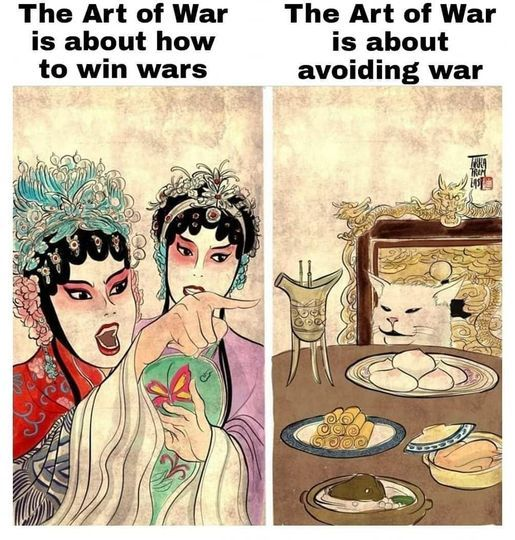
\includegraphics[width=5cm]{img/1651166248397.jpeg}~\\
	\end{column}
	\begin{column}[T]{7cm}
		\begin{itemize}
			\item Tester le processus de recrutement !
			\item Candidat myst{\`e}re : point de vue ext{\'e}rieur. 
			\item Pourquoi le candidat refuse ou ne r{\'e}pond plus ?
			\item Priorit{\'e}s du candidat ? (poste, localisation, r{\'e}mun{\'e}ration...)
			\item L'ordre des priorit{\'e}s est important !
			\item Ressenti d'int{\'e}r{\^e}t mutuel : le CV est-il lu avec attention ? 
		\end{itemize}
	\end{column}
	\end{columns}
	%% \begin{itemize}
	%%	\item Tester le processus de recrutement !~\newline
	%%		\texttt{https://www.linkedin.com/posts/activity-6925493203215245312-cR3U}~\newline
	%%		L'art de la guerre...~\newline
	%%		Parfois, au vus de certaines tentatives en mati{\`e}re de \#recrutement : cr{\'e}er une soci{\'e}t{\'e} de conseil pour le recrutement dans la tech ; un \#concept simple, des candidats myst{\`e}res se glissent dans votre processus de recrutement... \#startup \#conseil \#tech \#processus \#candidatmyst{\`e}re~\newline
	%%		De la m{\^e}me fa\c{c}on que des clients myst{\`e}res vont dans des magasins, restaurants, services... Et font ensuite un compte-rendu de fa\c{c}on anonyme, en g{\'e}n{\'e}ral via leur soci{\'e}t{\'e} ou entreprise (genre Gault et Millau, Guide du Routard, Guide Michelin...). Oui, cela existe encore ! \#GAFAM~\newline
	%%		Oui, de nombreuses entreprises auraient besoin de ce retour d'exp{\'e}rience de la part des candidats re\c{c}us ou contact{\'e}s pendant un recrutement, surtout dans "la tech" ! Et cela compte pour leur r{\'e}putation...~\newline
	%%		\#num{\'e}rique \#digital \#entreprises \#entreprise \#r{\'e}flexion
	%% \end{itemize} 
\end{frame}

\begin{frame}
	\frametitle{Autres id{\'e}es (En vrac - 2/9)}
	\begin{itemize}
		\item "Le recrutement, c'est comme la chasse : il y a les bons, les brutes et les truands !" (Le recrutement fonctionne mieux avec les bons !)
		\item Il ne faut pas que ce soit \emph{The Most Dangerous Game}, \emph{Battle Royale} ou \emph{Hunger Games} ! (Il y a des codes sociaux accept{\'e}s et des limites l{\'e}gales. )
		\item Demandez ce que les candidats pensent des recruteurs ! ("fraichement sorti d'{\'e}cole de commerce" ; "stagiaire" ;~\newline "recruteuse usant de (ses) charmes" ; "chasseur de pigeons" ;~\newline "la professionnelle", ... )
	\end{itemize}
	%% \begin{itemize}
	%% 	\item \texttt{https://www.linkedin.com/posts/activity-6932730981455949825-Tqwx}~\newline
	%% 		En mati{\`e}re de \#Recrutement, je songe {\`a} {\'e}crire un \#livre ou un \#JdR (au moins parodique) : il y a tellement {\`a} exprimer sur le sujet !~\newline
	%% 		Le commercial de "SSII / ESN du CAC 40" (oui, celle-l{\`a}) qui a probablement fait une {\'e}cole de commerce ; le stagiaire qui d{\'e}barque en RH...~\newline
	%% 		(le commercial d'{\'e}cole de commerce, le stagiaire qui d{\'e}barque, la "recruteuse" convaincue de ses charmes, le vendeur qui recherche des pigeons en demandant des r{\'e}f{\'e}rences, la RH professionnelle, le recruteur trop honn{\^e}te...).
	%% \end{itemize} 
\end{frame}

\begin{frame}
	\frametitle{Autres id{\'e}es (En vrac - 3/9)}
	%% ---
	\begin{columns}[T]
	\begin{column}[T]{5cm}
		
\includegraphics[width=5cm]{img/1655474560502.jpeg}~\\
	\end{column}
	\begin{column}[T]{7cm}
		~\\ \hfill ~\\
		La pissoti{\`e}re : le d{\'e}rangement doit valoir le co{\^u}t ! Sinon, c'est g{\^e}nant...~\\~\\~\\
		
		Laissez vos coordonn{\'e}es ; la relance c'est quand le processus de recrutement est d{\'e}j{\`a} entam{\'e} !
		%% ~\\ \hfill ~\\
	\end{column}
	\end{columns}
	%% \begin{itemize}
	%%	\item \texttt{https://www.linkedin.com/posts/activity-6943563576917807104-djRZ}~\newline
	%%		La pissoti{\`e}re : le d{\'e}rangement doit valoir le co{\^u}t ! Sinon, c'est g{\^e}nant...
	%% \end{itemize} 
\end{frame}

\begin{frame}
	\frametitle{Autres id{\'e}es (En vrac - 4/9)}
	\begin{columns}[T]
	\begin{column}[T]{5cm}
		
\includegraphics[width=5cm]{img/1657616562690.jpeg}~\\
	\end{column}
	\begin{column}[T]{7cm}
		\begin{itemize}
			\item Jusqu'o{\`u} aller pour recruter ? 
			\item La p{\^e}che au chalut ? La drague ? La prostitution ?
			\item {\`A} part pour le porno (films et produits d{\'e}riv{\'e}s) : utilit{\'e} du genre dans le recrutement ?
		\end{itemize}%% ~\\
		
\includegraphics[width=5cm]{img/1657616562426.jpeg}~\\
	\end{column}
	\end{columns}
	%% \begin{itemize}
	%%	\item \texttt{https://www.linkedin.com/posts/activity-6952547782712803328-t7Om}~\newline
	%%		On le rappelle : LinkedIn n'est pas Tinder ! Ah ben si en fait !
	%% \end{itemize} 
\end{frame}

\begin{frame}
	\frametitle{Autres id{\'e}es (En vrac - 5/9)}
	\begin{itemize}
		\item \textbf{Personnalisez les messages !}
		\item En soi, faire des messages g{\'e}n{\'e}rique est, peut-{\^e}tre, une bonne id{\'e}e ; 
			sauf pour les destinataires, qui n'auront aucune information (mission, poste, r{\'e}mun{\'e}ration...). 
		\item \textbf{Mod{\`e}le pr{\'e}-rempli ou {\`a} remplir : }
		\begin{itemize}
			\item Pourquoi cibler telle ou telle personne ?
			\item Descriptif de poste lisible rapidement !
			\item R{\'e}mun{\'e}ration ?!
		\end{itemize}
		%% \item \texttt{https://www.linkedin.com/posts/activity-6963075115613876224-uY\_J}~\newline
		%% 	Arr{\^e}tez les messages g{\'e}n{\'e}riques !~\newline
		%% 	Les messages de \#recrutement g{\'e}n{\'e}riques sur \#LinkedIn : tout un art ! Entre autre ici avec Extia~\newline
		%% 	C'est comme les lettres de \#motivation : le mod{\`e}le \#g{\'e}n{\'e}rique ou \#template vaut le co{\^u}t d'aller plus loin !~\newline
		%% 	Pourquoi mon profil ? Descriptif de poste ? R{\'e}mun{\'e}ration ? ...~\newline
		%% 	Idem Atos : les messages de recrutement g{\'e}n{\'e}riques ne sont pas appr{\'e}ci{\'e}s. Pour de bonnes raisons.~\newline
		%% 	\#Recrutement \#Num{\'e}rique '\#Digital' \#LinkedIn \#BonnesPratiques ...~\newline
		%% 	Qui r{\'e}pond encore ? Je n'aime ni le "name dropping" ni le "name shaming" : que faire contre ?~\newline
		%% 	Poke Devoteam \#recruteurs : pouvez vous mieux former vos recruteuses et recruteurs. Les messages g{\'e}n{\'e}riques de \#Recrutement \#IT : ce n'est pas en votre faveur ! Surtout en double ce matin.~\newline
		%% 	\#ESN \#SS2I \#LinkedIn ...~\newline
		%% 	Pour les autres soci{\'e}t{\'e}s de services aussi !
	\end{itemize} 
\end{frame}

\begin{frame}
	\frametitle{Autres id{\'e}es (En vrac - 6/9)}
	\begin{columns}[T]
	\begin{column}[T]{5cm}
		
\includegraphics[width=5cm]{img/1673900833331.jpeg}~\\
	\end{column}
	\begin{column}[T]{7cm}
		\begin{itemize}
			\item Le contenu du poste ?
			\item Et sa localisation ?
			\item Et la r{\'e}mun{\'e}ration ? (ni la visibilit{\'e} ni la passion)
		\end{itemize}%% ~\\
	\end{column}
	\end{columns}
	%% \begin{itemize}
	%%	\item \texttt{https://www.linkedin.com/posts/activity-7020848968561520641-lC2k}~\newline
	%%		\#Twitter : monde merveilleux o{\`u}, {\`a} l'image de la vraie vie, on peut trouver des critiques de \#LinkedIn et des m{\'e}thodes de \#Recrutement foireuses !~\newline
	%%		\#IRL \#R{\'e}seauxSociaux ...~\newline
	%%		Pr{\'e}sentez le contenu du poste ! Et poste r{\'e}aliste !
	%% \end{itemize} 
\end{frame}

\begin{frame}
	\frametitle{Autres id{\'e}es (En vrac - 7/9)}
	\begin{columns}[T]
	\begin{column}[T]{5cm}
		
\includegraphics[width=5cm]{img/1687203978939.jpeg}~\\
	\end{column}
	\begin{column}[T]{8cm}
		\begin{itemize}
			\item Le recrutement "efficace" de non-candidats pour les nuls.~\newline
			\item Lui proposer un poste sans d{\'e}crire la stack. 
			\item Lui proposer un poste {\`a} 200km. 
			\item Lui proposer un poste sous pay{\'e}.~\newline
			\item Perdu, rien de tout \c{c}a ne marche ! 
		\end{itemize}%% ~\\
	\end{column}
	\end{columns}
	%% \begin{itemize}
	%%	\item https://www.linkedin.com/posts/activity-7076646406790246400-c2Ac~\newline
	%%		Le recrutement "efficace" de non-candidats pour les nuls.~\newline
	%%		Lui proposer un poste sans d{\'e}crire la stack.~\newline
	%%		Lui proposer un poste {\`a} 200km.~\newline
	%%		Lui proposer un poste sous pay{\'e}.~\newline
	%%		Perdu, rien de tout \c{c}a ne marche dans la r{\'e}alit{\'e}. \#recrutement \#dev \#emploi \#travail \#informatique .~\newline
	%% \end{itemize} 
\end{frame}

\begin{frame}
	\frametitle{Autres id{\'e}es (En vrac - 8/9)}
	\begin{itemize}
		\item Int{\'e}ressez-vous {\`a} la culture des personn{\'e}es cibl{\'e}es ! 
		\item \c{C}a ne vous dit rien ? Heureusement, il y a \emph{Wikipedia}, \emph{WikiHow}, \emph{Wookiepedia}...
		\item Sinon, les moteurs de recherches peuvent r{\'e}pondre {\`a} vos questions, les personnes cibl{\'e}es aussi ; 
		\item Gothique, Chasseur ou Chasseuse de Pok{\'e}mon, Gameuse, R{\^o}liste, Intello ? ... 
		\item Et sinon, vous buvez quoi ? (r{\'e}ponses possibles : eau, th{\'e}, caf{\'e}, soda, autre). 
	\end{itemize}
	%% \begin{itemize}
	%% 	\item \texttt{https://www.linkedin.com/posts/activity-6980604583660118016--eer~}\newline
	%% 		Recrutement en \#informatique : \c{c}a se passe mieux quand il y a connaissance de la culture et des fa\c{c}ons de faire du \#num{\'e}rique !~\newline
	%% 		Am{\'e}lioration continue ? Culture ?~\newline
	%% 		\#RH \#PopCulture '\#digital' ...
	%% \end{itemize} 
\end{frame}

\begin{frame}
	\frametitle{Autres id{\'e}es (En vrac - 9/9)}
	\begin{columns}[T]
	\begin{column}[T]{5cm}
		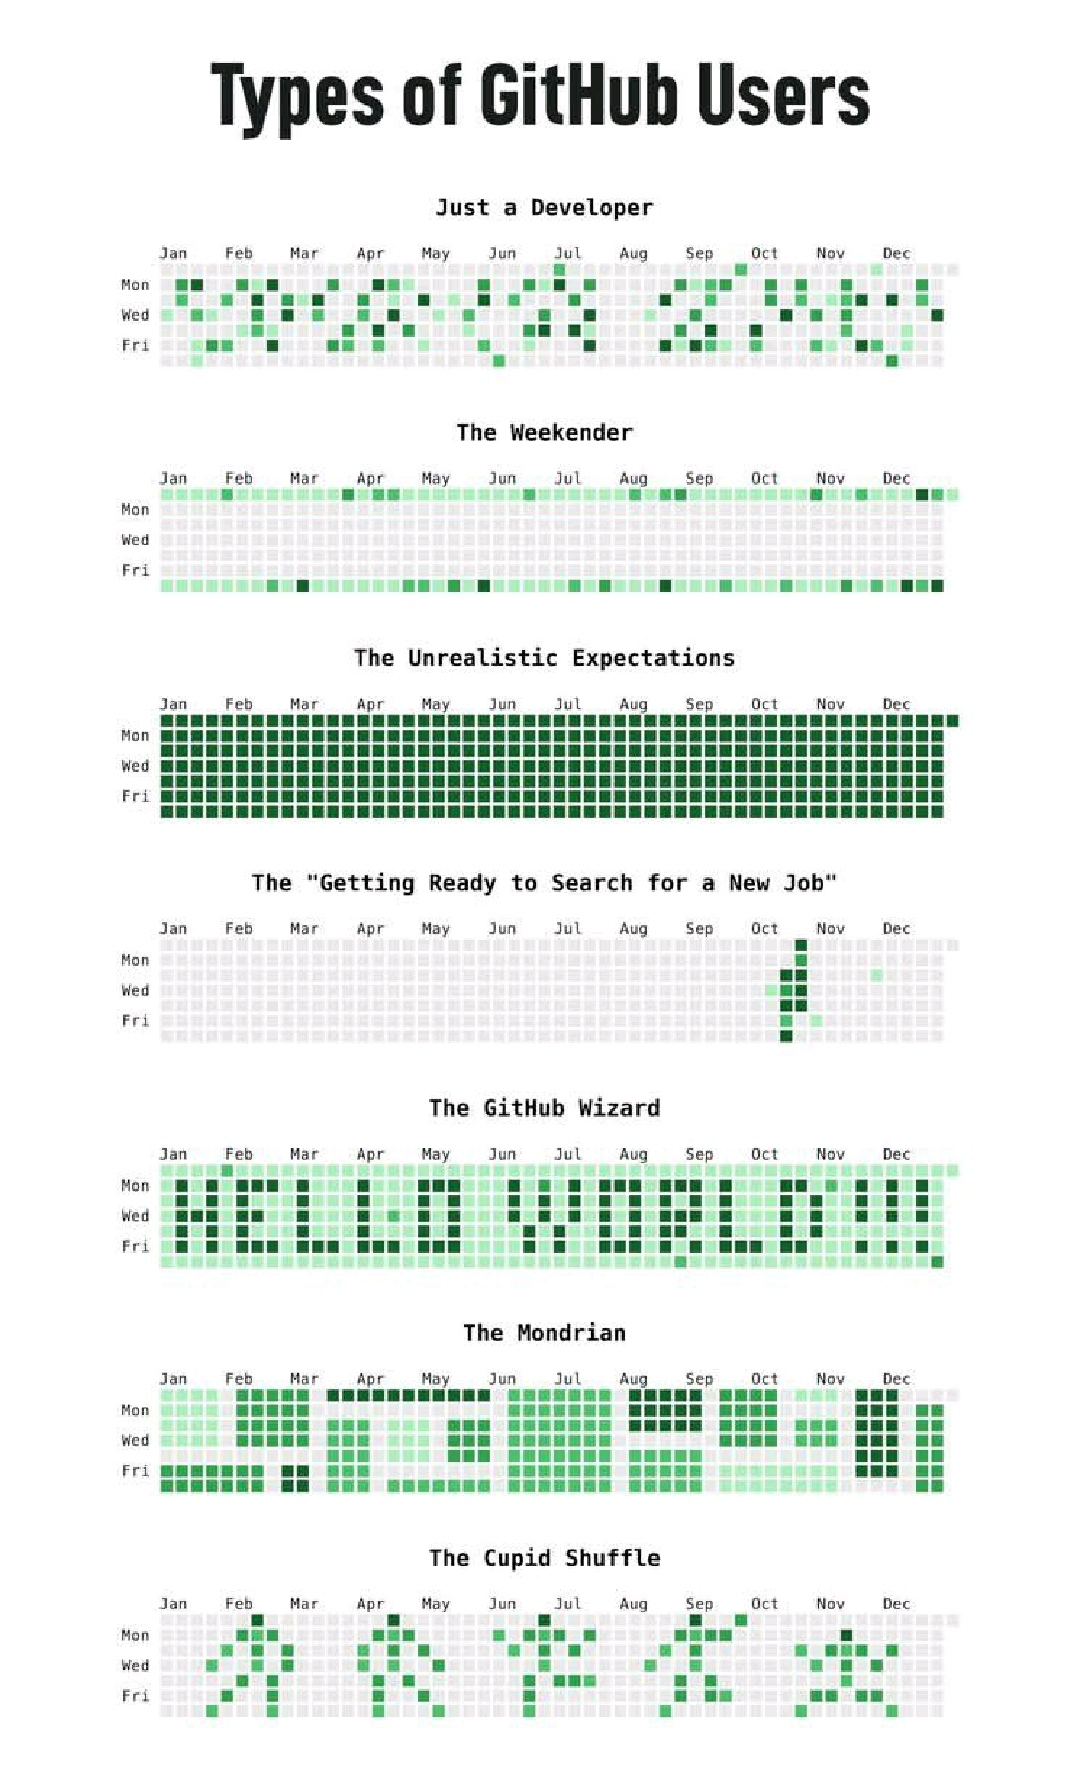
\includegraphics[width=4.15cm]{img/491521482-43a99eca-5204-4995-920f-dd18c0dcd2f0.jpg}~\\
	\end{column}
	\begin{column}[T]{7cm}
		\begin{itemize}
			\item Comprendre cet affichage, {\'e}vident pour beaucoup de d{\'e}veloppeurs !
			\item Qu'est-ce que vous comprenez ?
			\item Git / GitHub / GitLab ? "Demandez, Cherchez, Comprenez !"
			\item "Outil de versioning, code source, texte brut..." : outil et usages !
			\item R{\'e}f{\'e}rences autres : culturelles, sociales, fonctionnement humain... ? 
			\item ...
		\end{itemize}%% ~\\
	\end{column}
	\end{columns}
\end{frame}

%% \def\sectionPartBibliographie{Bibliographie / Mediagraphie}
%% \section{\sectionPartBibliographie}
%% \begin{frame}
%% 	\frametitle{\sectionPartBibliographie}
%% 	{\footnotesize 
%% 		\nocite{*}
%% 		%toutes references biblio : 6 lettres + 2 chiffres
%% 		\bibliography{presentationRecrutementInformatique}
%% 		% \bibliographystyle{frplain} % plain or frplain
%% 		\bibliographystyle{plain}
%% 	}
%% \end{frame}

\end{document}
